%% Standalone figure for the Statistical Mechanics exercises (Quiz 1).
%% Build: pdflatex quiz1_sol_profile.tex  (or run build.sh in this folder)
\documentclass[11pt,tikz,border=2pt]{standalone}
\usepackage{amsmath,amssymb}
\usetikzlibrary{arrows.meta, positioning}
\begin{document}
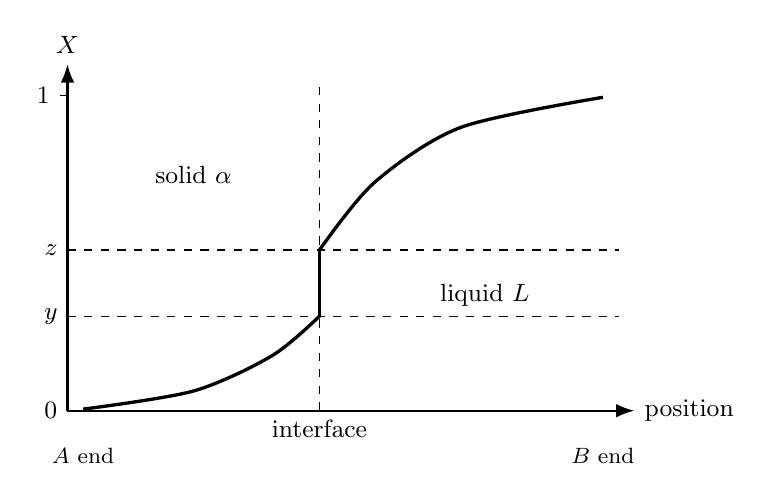
\begin{tikzpicture}[font=\small, >=Latex, line width=0.8pt]
    % axes: position along the couple, composition X
    \draw[->] (0,0) -- (7.2,0) node[right] {position};
    \draw[->] (0,0) -- (0,4.4) node[above] {$X$};
    \draw[line width=0.5pt] (0,4) -- (-0.1,4) node[left] {$1$};
    \node[left] at (0,0) {$0$};
    % compositions of the tie line at T_2
    \draw[dashed, line width=0.5pt] (0,1.2) node[left] {$y$} -- (7,1.2);
    \draw[dashed, line width=0.5pt] (0,2.04) node[left] {$z$} -- (7,2.04);
    % profile: alpha layer (0 -> y), jump at the interface, liquid (z -> 1)
    \draw[line width=1.2pt] plot[smooth] coordinates {(0.2,0.02) (1.6,0.25) (2.6,0.7) (3.2,1.2)};
    \draw[line width=1.2pt] (3.2,1.2) -- (3.2,2.04);
    \draw[line width=1.2pt] plot[smooth] coordinates {(3.2,2.04) (3.9,2.9) (5.0,3.6) (6.8,3.98)};
    \draw[dashed, line width=0.5pt] (3.2,0) node[below] {interface} -- (3.2,4.2);
    \node at (1.6,3.0) {solid $\alpha$};
    \node[above] at (5.3,1.2) {liquid $L$};
    \node[below, font=\footnotesize] at (0.2,-0.35) {$A$ end};
    \node[below, font=\footnotesize] at (6.8,-0.35) {$B$ end};
\end{tikzpicture}
\end{document}
